%%%%%%%%%%%%%%%%%%%%%%%%%%%%%%%%%%%%%%%%%
% Beamer Presentation
% LaTeX Template
% Version 1.0 (10/11/12)
%
% This template has been downloaded from:
% http://www.LaTeXTemplates.com
%
% License:
% CC BY-NC-SA 3.0 (http://creativecommons.org/licenses/by-nc-sa/3.0/)
%
%%%%%%%%%%%%%%%%%%%%%%%%%%%%%%%%%%%%%%%%%

%----------------------------------------------------------------------------------------
%	PACKAGES AND THEMES
%----------------------------------------------------------------------------------------

\documentclass{beamer}

\mode<presentation> {

% The Beamer class comes with a number of default slide themes
% which change the colors and layouts of slides. Below this is a list
% of all the themes, uncomment each in turn to see what they look like.

%\usetheme{default}
%\usetheme{AnnArbor}
%\usetheme{Antibes}
%\usetheme{Bergen}
%\usetheme{Berkeley}
%\usetheme{Berlin}
%\usetheme{Boadilla}
%\usetheme{CambridgeUS}
%\usetheme{Copenhagen}
%\usetheme{Darmstadt}
%\usetheme{Dresden}
%\usetheme{Frankfurt}
%\usetheme{Goettingen}
%\usetheme{Hannover}
%\usetheme{Ilmenau}
%\usetheme{JuanLesPins}
%\usetheme{Luebeck}
\usetheme{Madrid}
%\usetheme{Malmoe}
%\usetheme{Marburg}
%\usetheme{Montpellier}
%\usetheme{PaloAlto}
%\usetheme{Pittsburgh}
%\usetheme{Rochester}
%\usetheme{Singapore}
%\usetheme{Szeged}
%\usetheme{Warsaw}

% As well as themes, the Beamer class has a number of color themes
% for any slide theme. Uncomment each of these in turn to see how it
% changes the colors of your current slide theme.

%\usecolortheme{albatross}
%\usecolortheme{beaver}
%\usecolortheme{beetle}
%\usecolortheme{crane}
%\usecolortheme{dolphin}
%\usecolortheme{dove}
%\usecolortheme{fly}
%\usecolortheme{lily}
%\usecolortheme{orchid}
%\usecolortheme{rose}
%\usecolortheme{seagull}
%\usecolortheme{seahorse}
%\usecolortheme{whale}
%\usecolortheme{wolverine}

%\setbeamertemplate{footline} % To remove the footer line in all slides uncomment this line
%\setbeamertemplate{footline}[page number] % To replace the footer line in all slides with a simple slide count uncomment this line

%\setbeamertemplate{navigation symbols}{} % To remove the navigation symbols from the bottom of all slides uncomment this line
}

\usepackage{graphicx} % Allows including images
\DeclareGraphicsExtensions{.pdf,.png,.jpg}
\usepackage{booktabs} % Allows the use of \toprule, \midrule and \bottomrule in tables
\usepackage[skip = 2pt, font=scriptsize]{caption}
\usepackage{subfigure}

%----------------------------------------------------------------------------------------
%	TITLE PAGE
%----------------------------------------------------------------------------------------

\title[B Oscillation]{Measurement of the $B^0_s$ - $\bar{B}^0_s$ Oscillation Frequency} % The short title appears at the bottom of every slide, the full title is only on the title page

\author{Oliver Dahme} % Your name
\institute[UZH] % Your institution as it will appear on the bottom of every slide, may be shorthand to save space
{
University of Zurich \\ % Your institution for the title page
\medskip
\textit{o.dahme@cern.ch} % Your email address
}
\date{\today} % Date, can be changed to a custom date

\begin{document}

\begin{frame}
	\titlepage % Print the title page as the first slide
\end{frame}

% \begin{frame}
% \frametitle{Overview} % Table of contents slide, comment this block out to remove it
% \tableofcontents % Throughout your presentation, if you choose to use \section{} and \subsection{} commands, these will automatically be printed on this slide as an overview of your presentation
% \end{frame}

%----------------------------------------------------------------------------------------
%	PRESENTATION SLIDES
%----------------------------------------------------------------------------------------

%------------------------------------------------
\section{Introduction} % Sections can be created in order to organize your presentation into discrete blocks, all sections and subsections are automatically printed in the table of contents as an overview of the talk
%------------------------------------------------

\begin{frame}
	\frametitle{Abstract}
	\begin{itemize}
		\item first precise measurement of the $B^0_s$ - $\bar{B}^0_s$ oscillation frequency $\Delta m_s$
		\item 1$fb^{-1}$ of data from $p \bar{p}$ collisions at $\sqrt{s} = 1.96$ TeV
		\item 3600 fully reconstructed $B_s$ decays and 37000 partially reconstructed semileptonic $B_s$ decays
		\item $\Delta m_s = 17.31^{+0.33}_{-0.18} (stat) \pm 0.07 (syst) ps^{-1}$
		\item $V_{td} / V_{ts} = 0.208^{+0.001}_{-0.002}(expt) ^{+0.008}_{-0.006} (theor)$
	\end{itemize}
\end{frame}
%------------------------------------------------

\begin{frame}
	\frametitle{Theory}
	\begin{itemize}
		\item probability for a $\bar{B}^0_q$ produced at time $t=0$ to decay as a $B^0_q$ at time $t$
	\end{itemize}
	\begin{align*}
		P_\pm (t) = \frac{\Gamma_q}{2} e^{-\Gamma_q t} \left[1 \pm \cos(\Delta m_q t) \right]
	\end{align*}
	\begin{itemize}
		\item $\Delta m_q = $ mass difference between $B^0_{q,H}$ and $B^0_{q,L}$
		\item $\Gamma_q$ is the decay width
	\end{itemize}
\end{frame}

\begin{frame}
	\frametitle{Theory}
	\begin{figure}
		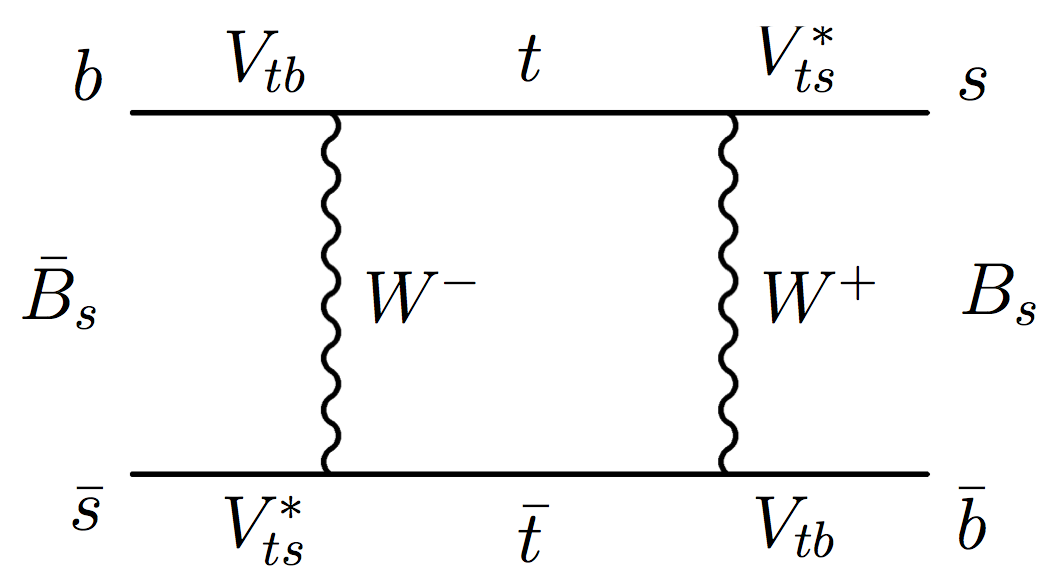
\includegraphics[width=0.75\textwidth]{B_mixing}
		\caption{Feynman Diagram of $B^0$ - $\bar{B}^0$ oscillation}
		\label{fig:mixing}
	\end{figure}
\end{frame}

%------------------------------------------------

\section{Experiment}
\begin{frame}
	\frametitle{Measurment method}
	\begin{itemize}
		\item 2 decay modes reconstructed:
		\item $\bar{B}^0_s \rightarrow D^+_s \pi^- , D^+_s \pi^- \pi^+ \pi^-$
		\item $\bar{B}^0_s \rightarrow D^+_s \ell^- \bar{\nu}_\ell, \ell = e$ or $\mu$
		\item using charged particles only
		\item calculating decay time from distance and momentum measurment between production and decay
		\item flavor at decay determined by charge of decay products
	\end{itemize}
\end{frame}

\begin{frame}
	\frametitle{Tagging initial B}
	\begin{itemize}
		\item 2 techniques to identify flavor of the B at production
		\item same-side tag: uses secondary meson $K^-$ for $\bar{B}^0_s$ and $K^+$ for $B^0_s$
		\item high sensitivity at large values of $\Delta m$
		\item opposite-side tag: uses charge of the lepton from the semileptonic decay
		\item high sensitivity at low values of $\Delta m$
	\end{itemize}
\end{frame}

\begin{frame}
	\frametitle{checking for unitarity of the CKM matrix}
	\begin{itemize}
		\item the measured oscillation frequency can be used to derive:
	\end{itemize}
	\begin{align*}
		\frac{V_{td}}{V_{ts}} = \epsilon \sqrt{\frac{\Delta m_d}{\Delta m_s} \frac{m_{B^0_s}}{m_{B^0}}} \sim 0.208
	\end{align*}
	\begin{itemize}
		\item which is consistent with standart model expectations
		\item can be used to improve constrains on the unitarity of the CKM matrix or on new physics
		\item it is still a topic in state of the art research at the LHCb experiment
	\end{itemize}
\end{frame}


%------------------------------------------------
\begin{frame}
	\frametitle{Questions?}
\end{frame}

%------------------------------------------------

%------------------------------------------------

%----------------------------------------------------------------------------------------

\end{document}
